\documentclass[border=4pt]{standalone}
\usepackage[T1]{fontenc}\usepackage{times}\usepackage[dvipsnames]{xcolor}\usepackage{tikz}
\usetikzlibrary{arrows.meta,positioning,shapes.geometric,fit}
\definecolor{dk}{RGB}{20,60,120}\definecolor{rd}{RGB}{170,30,30}\definecolor{gn}{RGB}{20,110,50}
\newcommand{\code}[1]{\texttt{\small #1}}
\begin{document}
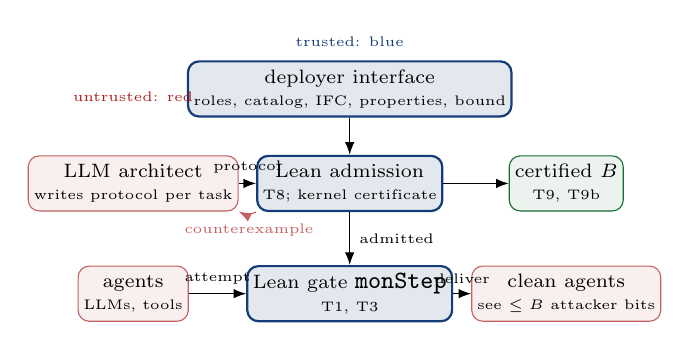
\begin{tikzpicture}[font=\scriptsize, box/.style={draw,rounded corners,align=center,minimum height=7mm,inner sep=2pt},
  trusted/.style={box,fill=dk!12,draw=dk,thick}, untr/.style={box,fill=rd!7,draw=rd!70}, ar/.style={-{Latex[length=1.6mm]}}]
\node[trusted] (pol) at (0,1.55) {deployer interface\\{\tiny roles, catalog, IFC, properties, bound}};
\node[untr] (arch) at (-2.75,0.35) {LLM architect\\{\tiny writes protocol per task}};
\node[trusted] (adm) at (0,0.35) {Lean admission\\{\tiny T8; kernel certificate}};
\node[untr] (ag) at (-2.75,-1.05) {agents\\{\tiny LLMs, tools}};
\node[trusted] (gate) at (0,-1.05) {Lean gate \code{monStep}\\{\tiny T1, T3}};
\node[untr] (cl) at (2.75,-1.05) {clean agents\\{\tiny see $\le B$ attacker bits}};
\node[box,draw=gn,fill=gn!8] (bits) at (2.75,0.35) {certified $B$\\{\tiny T9, T9b}};
\draw[ar] (pol) -- (adm); \draw[ar] (arch) -- node[above]{\tiny protocol} (adm);
\draw[ar,rd!70] (adm.south west) to[bend left=25] node[below,pos=0.4]{\tiny counterexample} (arch.south east);
\draw[ar] (adm) -- node[right]{\tiny admitted} (gate); \draw[ar] (ag) -- node[above]{\tiny attempt} (gate);
\draw[ar] (gate) -- node[above]{\tiny deliver} (cl); \draw[ar] (adm) -- (bits);
\node[font=\tiny,text=dk] at (0,2.15) {trusted: blue};\node[font=\tiny,text=rd] at (-2.75,1.45) {untrusted: red};
\end{tikzpicture}
\end{document}
